\chapter{THIẾT KẾ CƠ SỞ DỮ LIỆU}

\section{Sơ đồ Thực thể Liên kết (ERD) toàn hệ thống}
Cơ sở dữ liệu của hệ thống BrewLite được chuẩn hóa theo dạng chuẩn 3NF, thiết kế bám sát tập tin mô hình dữ liệu \texttt{backend/prisma/schema.prisma}. Toàn bộ hệ thống bao gồm 12 thực thể quan hệ, đảm bảo tính toàn vẹn dữ liệu, hiệu năng truy vấn và hỗ trợ chuyên sâu cho các nghiệp vụ phức tạp như kiểm soát đồng thời (Optimistic Locking) và thanh toán bất biến (Idempotency).

Sơ đồ ERD toàn hệ thống được trình bày ở chế độ khổ ngang (Landscape) tại Hình~\ref{fig:database-erd}.

\begin{landscape}
\begin{figure}[p]
    \centering
    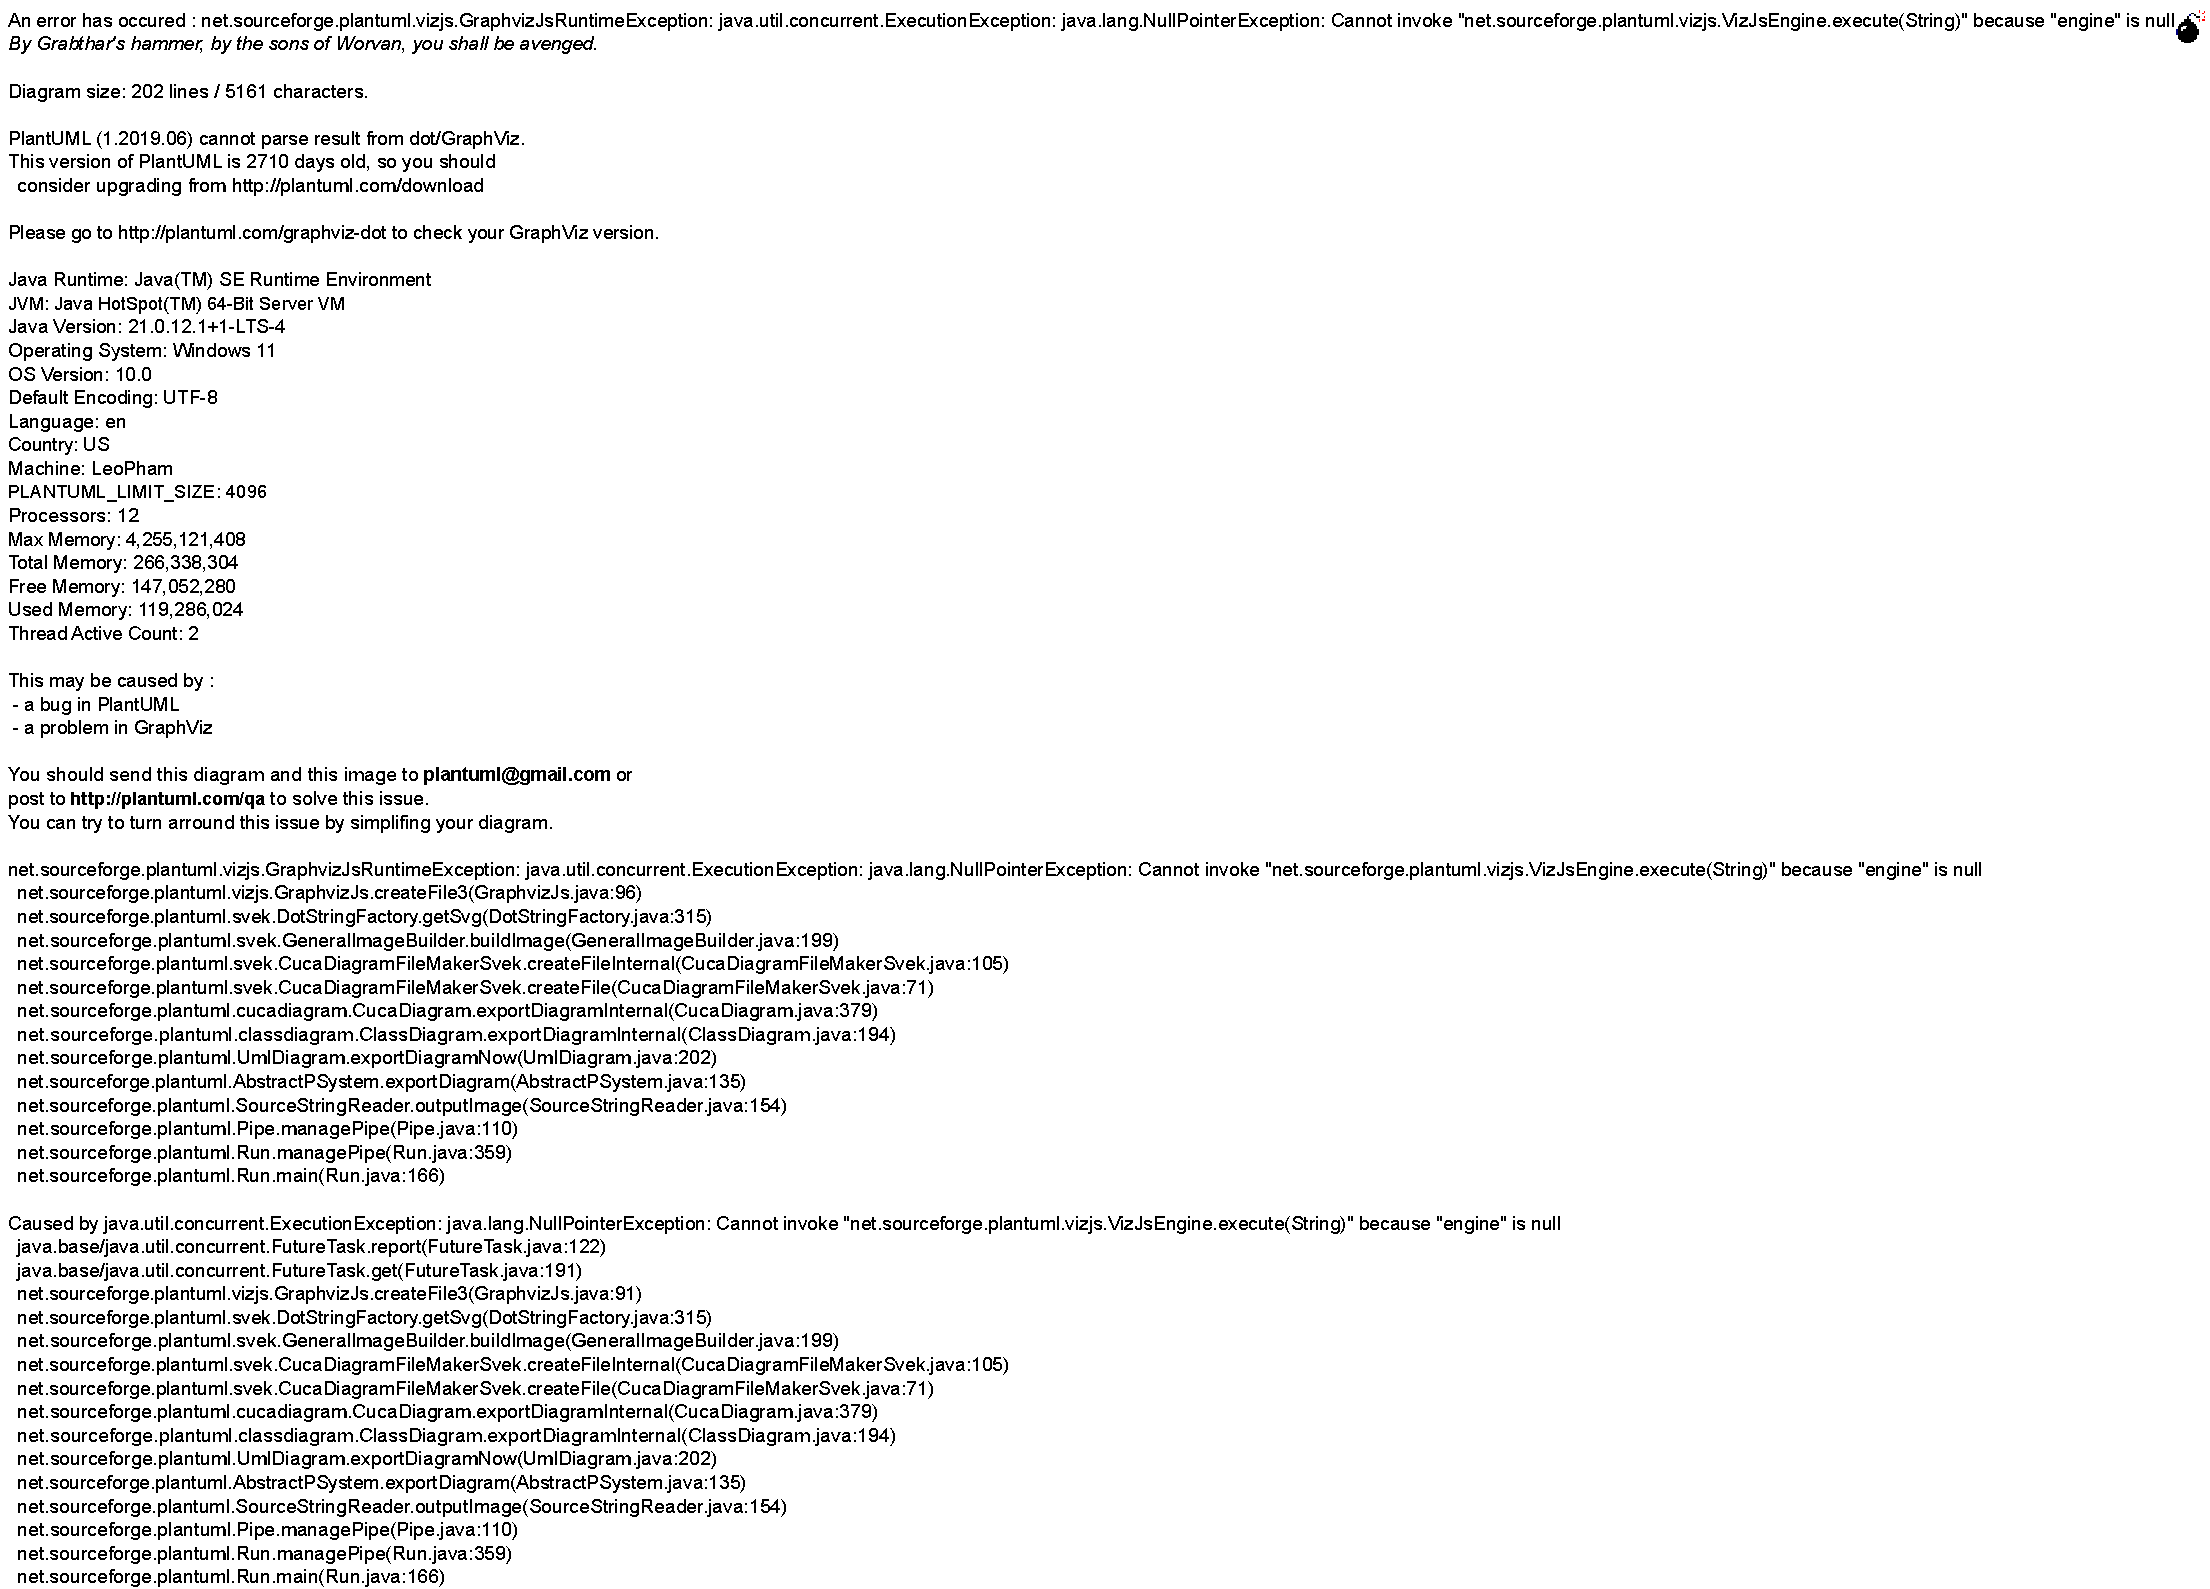
\includegraphics[width=0.98\linewidth,height=0.88\textheight,keepaspectratio]{figures/database-erd.pdf}
    \caption{Sơ đồ Thực thể Liên kết (ERD) toàn hệ thống BrewLite}
    \label{fig:database-erd}
\end{figure}
\end{landscape}

\section{Chi tiết 12 thực thể trong Cơ sở dữ liệu}
Mô hình dữ liệu bao gồm 12 bảng được phân chia theo các nhóm nghiệp vụ chính:

\begin{enumerate}
    \item \textbf{Nhóm Người dùng và Định danh:}
    \begin{itemize}
        \item \textbf{\texttt{users}:} Lưu trữ thông tin định danh khách hàng. Gồm các trường: \texttt{id} (PK, cuid), \texttt{email} (Unique, chuỗi định danh duy nhất), \texttt{password\_hash} (mật khẩu băm Bcrypt 10 rounds), \texttt{full\_name}, \texttt{loyalty\_points} (điểm tích lũy hiện có, mặc định 0), \texttt{created\_at}, \texttt{updated\_at}.
    \end{itemize}

    \item \textbf{Nhóm Danh mục và Sản phẩm:}
    \begin{itemize}
        \item \textbf{\texttt{categories}:} Phân loại thực đơn (Cà phê, Trà...). Gồm: \texttt{id} (PK), \texttt{name} (Unique), \texttt{slug} (Unique), \texttt{display\_order} (thứ tự hiển thị trên tab giao diện), \texttt{created\_at}, \texttt{updated\_at}.
        \item \textbf{\texttt{products}:} Thông tin đồ uống. Gồm: \texttt{id} (PK), \texttt{category\_id} (FK \(\to\) \texttt{categories.id}), \texttt{name}, \texttt{base\_price} (Decimal(12,0) tiền VNĐ nguyên chẵn), \texttt{image\_url}, \texttt{stock} (số lượng tồn kho khả dụng), \texttt{version} (Int, default 0 - trường phiên bản phục vụ Optimistic Locking), \texttt{is\_available} (Boolean), \texttt{created\_at}, \texttt{updated\_at}.
        \item \textbf{\texttt{product\_size_prices}:} Cấu hình phụ thu theo từng kích cỡ (S, M, L) cho từng sản phẩm. Gồm: \texttt{id} (PK), \texttt{product\_id} (FK \(\to\) \texttt{products.id}, Cascade), \texttt{size} (Enum \texttt{ProductSize}: S, M, L), \texttt{price\_adjustment} (Decimal(12,0)). Có ràng buộc duy nhất \texttt{@@unique([product\_id, size])}.
        \item \textbf{\texttt{toppings}:} Danh mục topping dùng kèm. Gồm: \texttt{id} (PK), \texttt{name} (Unique), \texttt{price} (Decimal(12,0)), \texttt{stock} (Int, default 100), \texttt{is\_available} (Boolean), \texttt{created\_at}, \texttt{updated\_at}.
    \end{itemize}

    \item \textbf{Nhóm Khuyến mãi (Promotions):}
    \begin{itemize}
        \item \textbf{\texttt{promotions}:} Quản lý mã giảm giá voucher. Gồm: \texttt{id} (PK), \texttt{code} (Unique, ví dụ: \texttt{WELCOME10}, \texttt{GIAM15K}), \texttt{description}, \texttt{discount\_percent} (tỷ lệ giảm theo \%), \texttt{discount\_amount} (tiền giảm cố định), \texttt{max\_discount} (mức giảm trần tối đa, ví dụ 20.000 VNĐ trong mã \texttt{WELCOME10}), \texttt{min\_order\_amount} (giá trị đơn tối thiểu, ví dụ 40.000 VNĐ trong mã \texttt{WELCOME10} hoặc 60.000 VNĐ trong mã \texttt{GIAM15K}), \texttt{start\_date}, \texttt{end\_date}, \texttt{is\_active} (Boolean).
    \end{itemize}

    \item \textbf{Nhóm Đơn hàng và Chi tiết:}
    \begin{itemize}
        \item \textbf{\texttt{orders}:} Bảng trung tâm lưu trữ thông tin đơn hàng. Gồm: \texttt{id} (PK), \texttt{order\_number} (Int, Unique, autoincrement - mã hiển thị cho khách dạng \#1042), \texttt{user\_id} (FK \(\to\) \texttt{users.id}), \texttt{promotion\_id} (FK \(\to\) \texttt{promotions.id}, có thể null), \texttt{status} (Enum \texttt{OrderStatus}), \texttt{total\_amount} (tạm tính trước giảm), \texttt{discount\_amount} (số tiền được giảm), \texttt{final\_amount} (số tiền thực trả), \texttt{points\_earned} (số điểm thưởng tích được từ đơn), \texttt{paid\_at} (thời điểm thanh toán), \texttt{version} (Int, default 0 - Optimistic Locking khi chuyển trạng thái), \texttt{created\_at}, \texttt{updated\_at}.
        \item \textbf{\texttt{order\_items}:} Chi tiết từng món trong đơn. Gồm: \texttt{id} (PK), \texttt{order\_id} (FK \(\to\) \texttt{orders.id}, Cascade), \texttt{product\_id} (FK \(\to\) \texttt{products.id}), \texttt{size} (Enum \texttt{ProductSize}), \texttt{quantity} (Int), \texttt{unit\_price} (Decimal(12,0) - đơn giá snapshot đã cộng phụ thu size), \texttt{line\_total} (Decimal(12,0) = (unitPrice + toppings) \(\times\) quantity).
        \item \textbf{\texttt{order\_item\_toppings}:} Lưu trữ topping kèm theo từng món. Gồm: \texttt{id} (PK), \texttt{order\_item\_id} (FK \(\to\) \texttt{order\_items.id}, Cascade), \texttt{topping\_id} (FK \(\to\) \texttt{toppings.id}), \texttt{price} (Decimal(12,0) - snapshot giá topping tại thời điểm đặt).
        \item \textbf{\texttt{order\_status_history}:} Lưu vết lịch sử chuyển đổi trạng thái đơn hàng (phục vụ giám sát 9 chuyển tiếp của máy trạng thái). Gồm: \texttt{id} (PK), \texttt{order\_id} (FK \(\to\) \texttt{orders.id}, Cascade), \texttt{from\_status} (OrderStatus?), \texttt{to\_status} (OrderStatus), \texttt{changed\_by} (String?), \texttt{reason} (String?), \texttt{created\_at}.
    \end{itemize}

    \item \textbf{Nhóm Thanh toán và Điểm thành viên:}
    \begin{itemize}
        \item \textbf{\texttt{payments}:} Lưu thông tin các lần thanh toán. Gồm: \texttt{id} (PK), \texttt{order\_id} (FK \(\to\) \texttt{orders.id}, quan hệ 1-N hỗ trợ retry khi thanh toán thất bại), \texttt{idempotency\_key} (Unique, chuỗi UUID chống trùng lặp), \texttt{request\_hash} (mã băm SHA-256 nội dung request), \texttt{amount} (Decimal(12,0)), \texttt{method} (Enum: \texttt{BANK\_CARD}, \texttt{E\_WALLET}), \texttt{status} (Enum: \texttt{PENDING}, \texttt{SUCCESS}, \texttt{FAILED}), \texttt{failure\_reason}, \texttt{transaction\_ref}, \texttt{created\_at}.
        \item \textbf{\texttt{loyalty\_transactions}:} Nhật ký biến động điểm thưởng. Gồm: \texttt{id} (PK), \texttt{user\_id} (FK \(\to\) \texttt{users.id}), \texttt{order\_id} (FK \(\to\) \texttt{orders.id}?), \texttt{points} (Int), \texttt{type} (Enum: \texttt{EARNED}, \texttt{SPENT}, \texttt{REFUNDED}), \texttt{reason}, \texttt{created\_at}.
    \end{itemize}
\end{enumerate}

\section{Ràng buộc toàn vẹn và Chiến lược đánh chỉ mục}
\begin{itemize}
    \item \textbf{Ràng buộc Khóa ngoại (Referential Integrity):} Sử dụng cơ chế \texttt{onDelete: Cascade} cho các quan hệ cha-con gắn kết chặt chẽ: khi xóa đơn hàng (\texttt{Order}), hệ thống tự động dọn dẹp các dòng tương ứng trong \texttt{order\_items}, \texttt{order\_item\_toppings}, \texttt{order\_status\_history} và \texttt{payments}. Ngược lại, quan hệ giữa \texttt{Product} và \texttt{OrderItem} áp dụng cơ chế bảo vệ (\texttt{Restrict}) để ngăn ngừa việc xóa mất dấu sản phẩm đã có trong hóa đơn.
    \item \textbf{Ràng buộc Duy nhất (Unique Constraints):} Thiết lập chỉ mục duy nhất trên \texttt{users(email)}, \texttt{categories(slug)}, \texttt{categories(name)}, \texttt{promotions(code)}, \texttt{orders(order\_number)}, \texttt{payments(idempotency\_key)} và bộ đôi \texttt{product\_size\_prices(product\_id, size)}.
    \item \textbf{Chỉ mục Tối ưu truy vấn (Query Optimization Indexes):} Đánh chỉ mục B-tree trên các trường khóa ngoại và các trường thường xuyên xuất hiện trong mệnh đề lọc/sắp xếp:
    \begin{itemize}
        \item \texttt{orders(user\_id)}, \texttt{orders(status)}: tăng tốc độ truy vấn danh sách lịch sử đơn hàng.
        \item \texttt{order\_items(order\_id)}: tăng tốc độ nạp dữ liệu hóa đơn chi tiết.
        \item \texttt{payments(order\_id)}: hỗ trợ tra cứu các giao dịch theo đơn hàng.
        \item \texttt{loyalty\_transactions(user\_id)}: tối ưu hóa việc tính toán lịch sử điểm thưởng.
    \end{itemize}
\end{itemize}

\section{Thiết kế CSDL hỗ trợ nghiệp vụ nâng cao}
Cơ sở dữ liệu của BrewLite được tính toán kỹ lưỡng ngay từ thiết kế schema để đáp ứng các bài toán kỹ thuật phức tạp:
\begin{enumerate}
    \item \textbf{Kiểm soát Đồng thời (Optimistic Locking):} Trường \texttt{version} trên bảng \texttt{products} và \texttt{orders} cho phép phát hiện xung đột dữ liệu mà không cần khóa bi quan (Pessimistic lock) gây nghẽn cổ chai. Câu lệnh cập nhật kho luôn đi kèm điều kiện \texttt{WHERE id = :id AND version = :currentVersion}, tự động tăng \texttt{version = version + 1}.
    \item \textbf{Thanh toán Bất biến (Idempotent Payment):} Trường \texttt{idempotency\_key} có tính duy nhất toàn cục kết hợp cùng \texttt{request\_hash} trong bảng \texttt{payments} giúp hệ thống ngay lập tức nhận diện các request gửi lại từ client hoặc lỗi mạng, trả về kết quả đã xử lý mà không thực hiện gọi lại cổng thanh toán.
    \item \textbf{Snapshot Lịch sử Giá (Price Immutability):} Các trường \texttt{unit\_price} trong \texttt{order\_items} và \texttt{price} trong \texttt{order\_item\_toppings} sao lưu chính xác giá trị tại thời điểm khách hàng đặt, đảm bảo giá trị hóa đơn luôn cố định bất biến theo thời gian.
\end{enumerate}
